\documentclass[12pt]{article}
\usepackage[top=1in,left=1in, right = 1in, footskip=1in]{geometry}

\usepackage{graphicx}
%\usepackage{adjustbox}

%% \newcommand{\comment}{\showcomment}
\newcommand{\comment}{\nocomment}

\newcommand{\showcomment}[3]{\textcolor{#1}{\textbf{[#2: }\textsl{#3}\textbf{]}}}
\newcommand{\nocomment}[3]{}

\newcommand{\jd}[1]{\comment{cyan}{JD}{#1}}
\newcommand{\swp}[1]{\comment{magenta}{SWP}{#1}}

\newcommand{\eref}[1]{(Eq.~\ref{eq:#1})}
\newcommand{\fref}[1]{Fig.~\ref{fig:#1}}
\newcommand{\Fref}[1]{Fig.~\ref{fig:#1}}
\newcommand{\sref}[1]{Sec.~\ref{#1}}
\newcommand{\frange}[2]{Fig.~\ref{fig:#1}--\ref{fig:#2}}
\newcommand{\tref}[1]{Table~\ref{tab:#1}}
\newcommand{\tlab}[1]{\label{tab:#1}}
\newcommand{\seminar}{SE\mbox{$^m$}I\mbox{$^n$}R}

\usepackage{amsthm}
\usepackage{amsmath}
\usepackage{amssymb}
\usepackage{amsfonts}

% \usepackage{lineno}
% \linenumbers

\usepackage[pdfencoding=auto, psdextra]{hyperref}

\usepackage{natbib}
\bibliographystyle{chicago}
\date{\today}

\usepackage{xspace}
\newcommand*{\ie}{i.e.\@\xspace}

\usepackage{color}

\newcommand{\Rx}[1]{\ensuremath{{\mathcal R}_{#1}}} 
\newcommand{\Ro}{\Rx{0}}
\newcommand{\RR}{\ensuremath{{\mathcal R}}}
\newcommand{\Rhat}{\ensuremath{{\hat\RR}}}
\newcommand{\tsub}[2]{#1_{{\textrm{\tiny #2}}}}

\begin{document}

\begin{flushleft}{
	\Large
	\textbf\newline{
		Biases in early-outbreak estimates of epidemiological delay distributions: applications to COVID-19 outbreak
	}
}
\end{flushleft}

\section*{Abstract}

\pagebreak

\section{Introduction}

Since the emergence of the novel coronavirus disease (COVID-19), a significant amount of research has been put into estimating the associated time delays between epidemiological events.
These events can be compared within an infected individual or between transmission pairs.
For example, key distributions for understanding the spread of COVID-19 include:
\begin{enumerate}
  \item Incubation period distribution: time between infection and symptom onset \citep{backer2020incubation, li2020early, linton2020incubation, tian2020characteristics}
  \item Serial interval distribution: time between symptom onset of an infector and an infectee \citep{du2020serial, nishiura2020serial, zhao2020estimating}
  \item Generation interval distribution: time between infection of an infector and an infectee \citep{ganyani2020estimating}
\end{enumerate}
The inferred delay distributions have been incorporated into modeling studies to estimate the epidemic potential of COVID-19 and assess the effectiveness of intervention strategies.

Measuring a delay between two epidemiological events depends on having observed both events.
A delay between two events cannot be measured if the second event has not occurred or has not been observed yet.
Here, we show that this dependency can systematically bias the estimate of a delay distribution if it is not explicitly taken into account;
this bias applies to \emph{all} epidemiological delay distributions.
We compare two approaches for correcting the bias and apply them to evaluate the amount of bias present in the early-outbreak estimate of the mean incubation period.

\section{Theoretical framework}

We begin by modeling epidemiological delays from a cohort perspective.
A ``cohort'' consists of all individuals whose first epidemiological event of interest occurred at a given time.
For example, for the purpose of measuring the duration of symptoms, cohort $s$ consists of all individuals who became symptomatic at time $s$.

Observed delay distributions are generally subject to ``right-censoring''.
Since events must occur before the time of measurement to be observed, delays in cohort $s$ that are longer than $t-s$ cannot be observed at time $t$.
Therefore, the cohort delay distribution $c_s(\tau|t)$ can be expressed as a truncated distribution:
\begin{equation}
c_s(\tau|t) = \frac{f_s(\tau)}{F_s(t-s)},\quad \tau \leq t-s
\end{equation}
where $f_s(\tau)$ is the ``true'' delay distribution and $F_s(\tau)$ is the corresponding cumulative distribution function.
Delay distributions involving more than one individual typically vary across cohorts with disease dynamics. For example, generation intervals will be shorter when the number of susceptibles is decreasing rapidly, since there will be fewer infection opportunities as the cohort grows older \citep{champredon2015intrinsic}.
Within-individual delay distributions that depend on external factors (e.g., time between symptom onset and hospitalization) can also change over time.

\begin{figure}[!th]
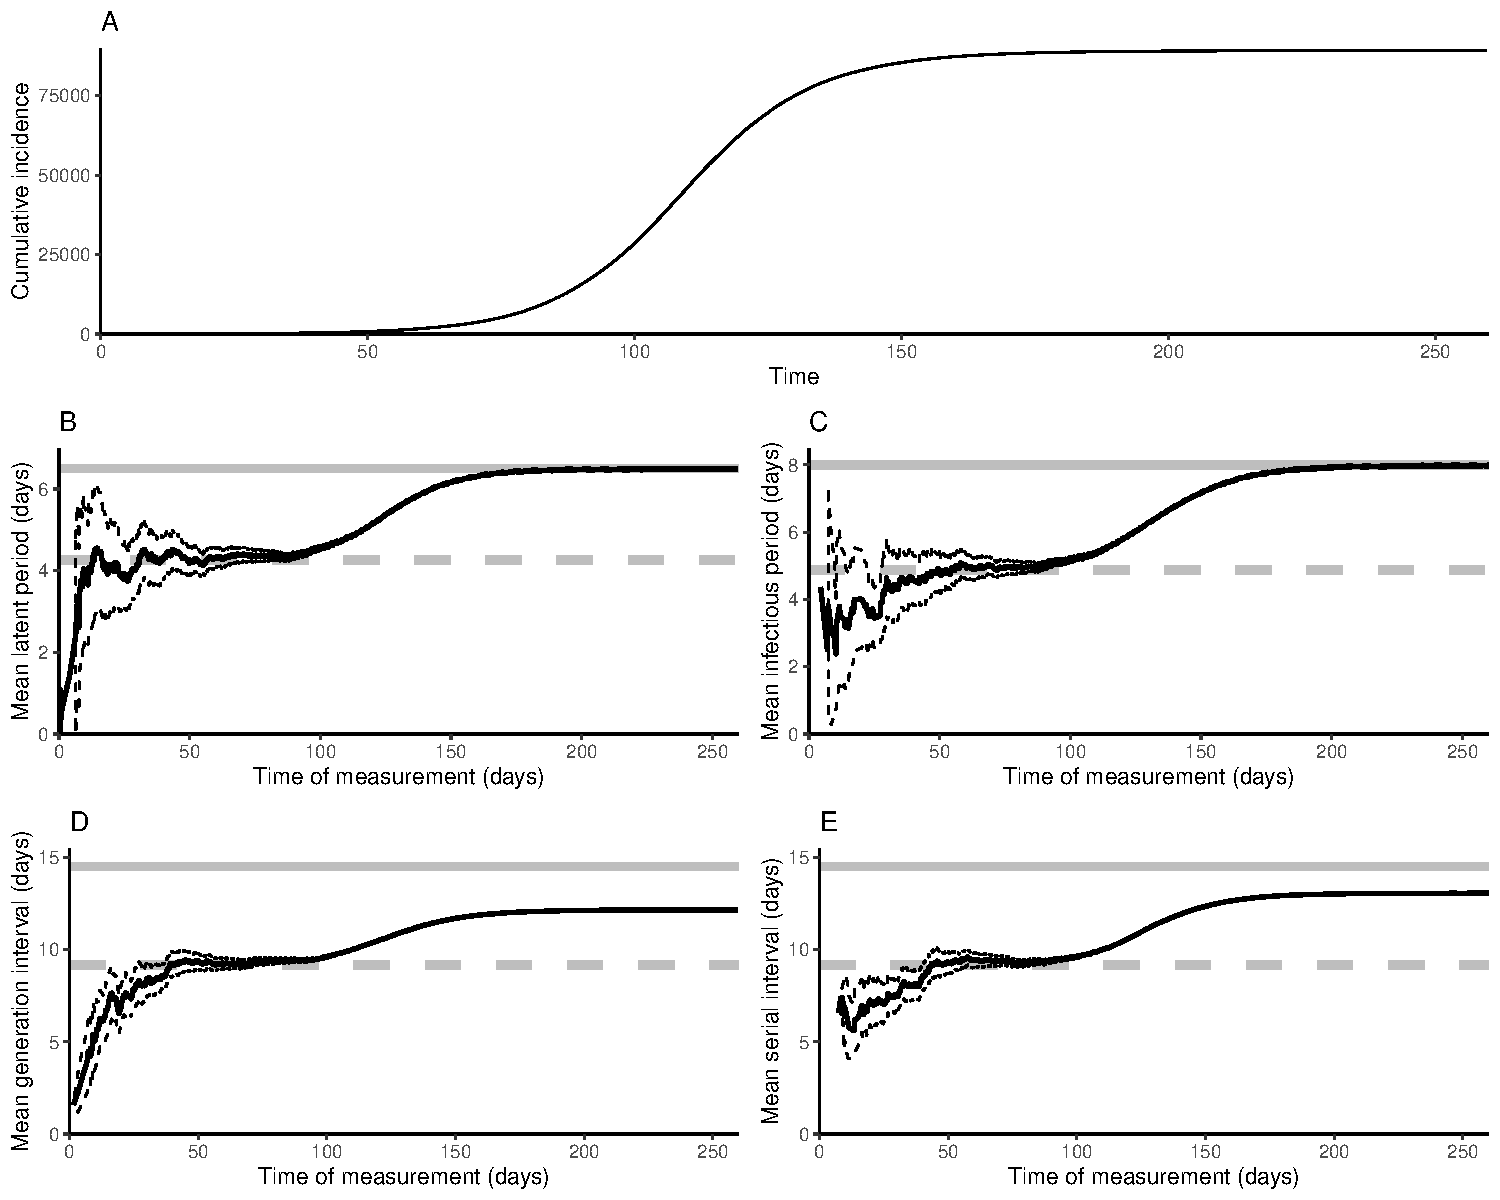
\includegraphics[width=\textwidth]{figure_seir.pdf}
\caption{
\textbf{Observed means of epidemiological delay distributions over time.}
Changes in the observed mean latent period (A), infectious period (B), generation interval (C), and serial interval (D) over the course of an epidemic.
Black solid lines represent the observed means and associated 95\% confidence intervals, which are calculated by taking all samples until the time of measurement $t$.
Gray solid lines represent the true mean.
Gray dashed lines represent the expected mean during the exponential growth phase (see \eref{exp}).
A stochastic SEIR model was simulated using a COVID-like parameters: $\mathcal R_0 = 2.5$, $1/\sigma = 6.5\,\textrm{days}$, $1/\gamma = 8\,\textrm{days}$, $N=100000$, and $I(0)=10$.
}
\label{fig:seir}
\end{figure}

Typically, epidemiological delay distributions are estimated by using \emph{all} available measured samples.
Then, the observed delay distribution $f_{\tiny\textrm{obs}}(\tau|t)$, which takes into account all measured delays until time $t$, can be expressed as an average of the cohort delay distributions $c_s(\tau|t)$, weighted by the size of cohorts $i(s)$ and the probability that both epidemiological events of interest will occur between time $s$ and $t$:
\begin{equation}
\begin{aligned}
f_{\tiny\textrm{obs}}(\tau|t) &\propto \int_{-\infty}^{t-\tau} c_s(\tau|t) i(s) F_s(t-s) ds\\
&= \int_{-\infty}^{t-\tau} i(s) f_s(\tau) ds
\end{aligned}
\end{equation}

Early in an epidemic, the incidence of infection, and therefore the size of cohorts, is expected to grow exponentially at rate $r > 0$: $i(s) \propto \exp(rs)$.
If cohort size is growing exponentially, we expect right censoring to be important: in other words, for fast-growing epidemics (high $r$), there will be a strong bias to observe shorter intervals.
This effect is shown in \fref{seir}. 
Stochastic simulations show that observed mean latent period, infectious period, generation interval, and serial interval increase through time. 
Eventually, the observed mean latent and infectious periods (but not the serial interval or generation interval) become unbiased.

% \jd{I took out a parenthetic comment about assumptions for the SI; it seemed out of place. We should probably introduce these intervals in the introduction.}

We can estimate the bias due to exponential growth.
Assuming that the true delay distribution stays constant during this period ($f_s(\tau) = f(\tau)$), 
the observed delay distribution during the exponential growth phase $f_{\tiny\textrm{exp}}(\tau|t)$ is equivalent to the true distribution weighted by the inverse of the exponential growth rate \citep{britton2019estimation}:
\begin{equation}
\begin{aligned}
f_{\tiny\textrm{exp}}(\tau|t) &\propto f(\tau) \int_{-\infty}^{t-\tau} \exp(rs) ds\\
&\propto f(\tau) \exp(-r\tau) \\
\end{aligned}
\end{equation}
These estimates are shown by the dashed grey lines in \fref{seir}: after initial transients, the observed means converge toward the expected exponential-growth values before increasing again as the epidemic no longer grows exponentially. % \jd{Should we show a time series of our simulated epidemic?}

The observed mean generation and serial intervals remain biased even at the end of the epidemic because the realized generation intervals become shorter due to susceptible depletion \citep{champredon2015intrinsic}.
The susceptible depletion effect can even occur at a finer, local scale (cf. \cite{park2019inferring})
% \jd{Maybe move this s.\ to Discussion; not here, I think.}.
The observed mean serial interval is slightly higher than the observed mean generation interval near the end of an epidemic because an infected individual with a short latent period (and shorter incubation period) is more likely infect others by transmitting faster (therefore, shorter generation interval) during the susceptible depletion phase; therefore, infectors are more likely to have shorter latent/incubation periods than their infectees.
Intervention strategies are also likely to introduce bias towards shorter generation and serial intervals because faster transmission events (i.e., shorter generation intervals) will be more likely to evade intervention.
% \jd{This whole \P\ is cool, but maybe a little deep. The last s.\ is also a bit terse; what effects do we expect? Similar between GI and SI, or similar to the previous s.?}

\begin{figure}[!th]
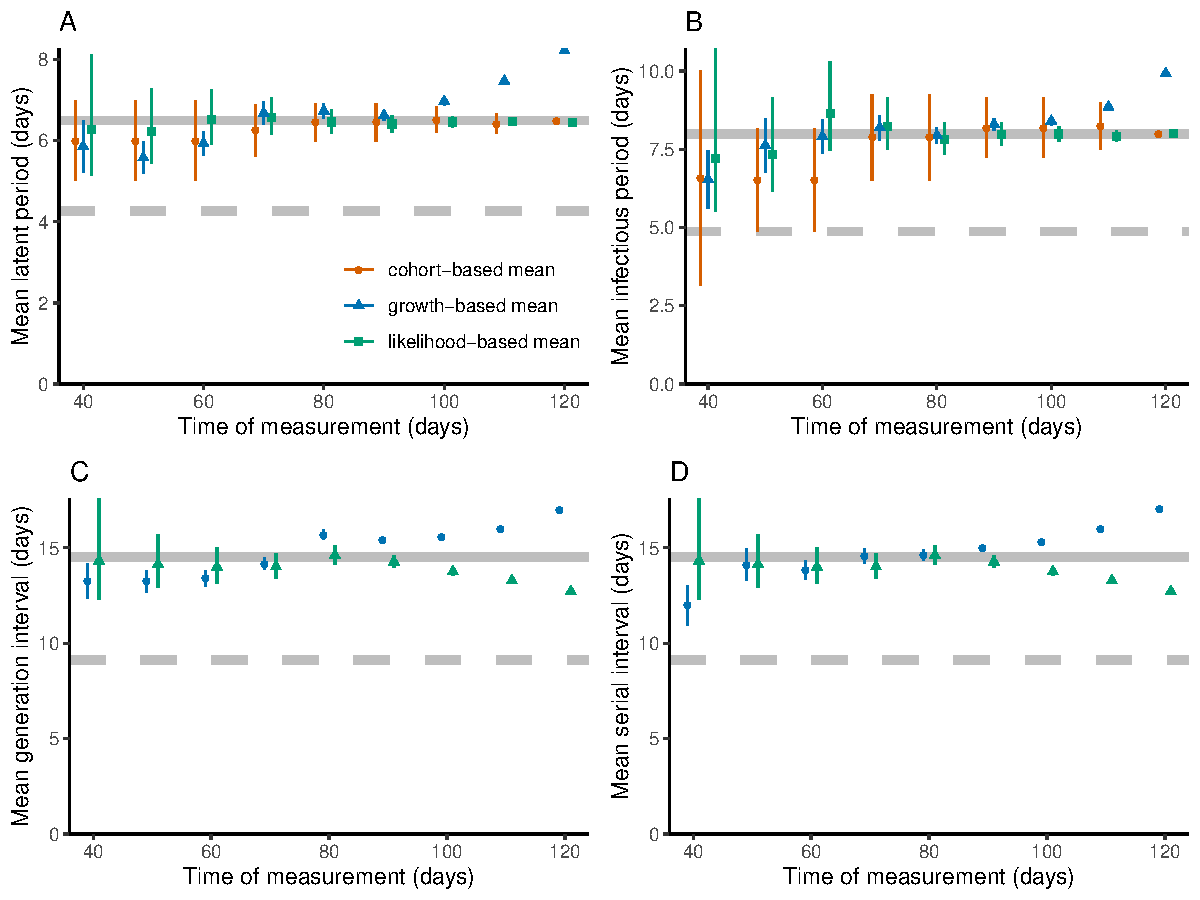
\includegraphics[width=\textwidth]{figure_seir2.pdf}
\caption{
\textbf{Estimated means of epidemiological delay distributions over time.}
Changes in the estimated mean latent period (A), infectious period (B), generation interval (C), and serial interval (D) over the course of an epidemic.
Blue solid lines represent the estimated mean and associated 95\% confidence intervals at each time of measurement using the growth-based approach.
Red solid lines represent the estimated mean and associated 95\% confidence intervals at each time of measurement using the cohort-based approach.
Gray solid lines represent the true mean.
Gray dashed lines represent the expected observed mean during the exponential growth phase calculated using Equation~\eref{exp}.
A stochastic SEIR model was simulated using the following parameters: $\mathcal R_0 = 2.5$, $1/\sigma = 6.5\,\textrm{days}$, $1/\gamma = 8\,\textrm{days}$, $N=50000$, and $I(0)=10$.
}
\label{fig:seir2}
\end{figure}

Equation~\eref{exp} suggests a seemingly straightforward way of correcting the bias -- by weighting the observed distribution by the exponential growth rate:
\begin{equation}
\label{eq:exp}
f(\tau) = f_{\tiny\textrm{exp}}(\tau|t) \exp(r \tau).
\end{equation}
Similar forms have been suggested by other studies \citep{britton2019estimation, park2019inferring} and have been applied in estimating epidemiological delay distributions during the COVID-19 outbreak \citep{nishiura2020serial, linton2020incubation};
however, our simulations show that the growth-based approach does not work very well for estimating the mean delay (\fref{seir2}).
Although the estimated mean delay is consistent with true mean, the estimates are unstable and the associated confidence intervals are inappropriately narrow.
Once the exponential growth phase is over, the assumptions of the growth-based approach no longer apply, and it becomes inconsistent.

% \jd{I would like to discuss this. We've talked before about throwing out that much information. How does the discarding method compare with the likelihood methods? The current text is a bit cryptic.}

Alternatively, we can account for the bias by ensuring that the right-censoring does not exist in the sample:
instead of using all samples that have been collected until the time of measurement, we can limit our samples to cohort $u < t$ such that both epidemiological events of interest have been observed for all individuals within cohorts $s < u$.
This approach provides an unbiased estimate of the mean delay throughout the epidemic with appropriately wide confidence intervals that contain the true value (\fref{seir2});
conversely, the proportion of individuals that have not completed the second event within each cohort will be indicative of the amount of bias present in the estimate.
This approach cannot be applied to generation or serial intervals because we don't know how many individuals each person infected exactly (and therefore we cannot evaluate whether the right-censoring exists within a cohort).
Nonetheless, likelihood-based methods that explicitly account for the right-censoring can be still applied to estimate the generation interval distribution \citep{park2019inferring}.

\section{Applications: incubation period distribution of COVID-19}

Here, we revisit the mean incubation period estimated by \cite{backer2020incubation} and assess the degree of potential bias in this estimate.
The estimate is based on travelers leaving Wuhan between January 2--23, during which the epidemic was likely to have been growing exponentially; it is reasonable to assume that the number of infected travelers was likely to have been increasing exponentially as well.
Therefore, their estimate of the mean \emph{observed} incubation periods of 6.4 days (95\% CI: 5.6–7.7 days) may be biased due to right-censoring.
To assess the presence of bias, we apply their method to infer infection time for each traveler and compare growth- and cohort-based means with the observed means over time.

\begin{figure}[!th]
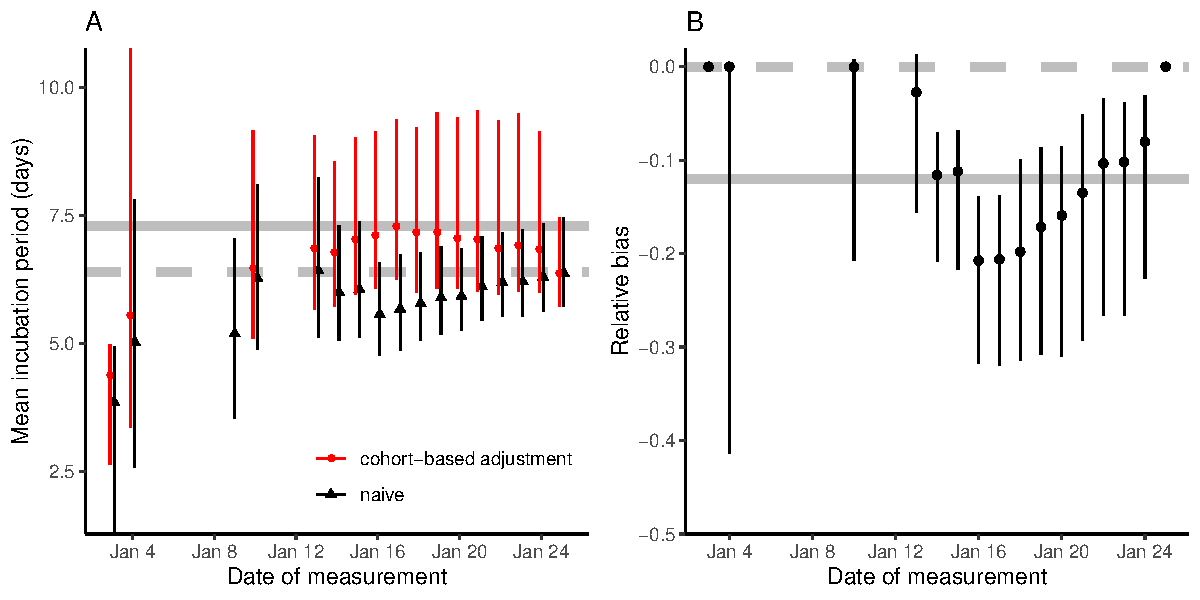
\includegraphics[width=\textwidth]{figure_baker.pdf}
\caption{
\textbf{Potential bias in the early-outbreak estimate of the mean incubation period.}
(A) Comparisons of the observed mean incubation period using all available samples and the cohort-based mean incubation period.
Gray solid line represents the growth-based mean incubation period.
Gray dashed line represents the mean incubation period estimated by \cite{backer2020incubation}.
(B) Relative bias of the mean observed incubation period with respect to the cohort-based mean incubation period.
Gray solid line represents relative bias with respect to the growth-based mean incubation period.
Gray dashed line represents the $y=0$ line.
Relative bias is calculated as $\textrm{(observed mean incubation period)/(bias-corrected mean incubation period)} - 1$.
}
\label{fig:backer}
\end{figure}

\fref{backer}A compares the observed mean incubation period, which uses all available measurements, with the cohort-based mean incubation period (see Methods for details of this section).
Consistent with our simulations, the cohort-based means are generally higher and have wider confidence intervals (see January 13--24 in \fref{backer}A).
For example, on January 24, the cohort-based mean incubation period is 6.9 days (95\% CI: 6.0 -- 9.1 days), whereas the observed mean incubation period is 6.3 days (95\% CI: 5.6 days -- 7.4 days).
The cohort-based mean also matches the growth-based mean: 7.3 days (95\% CI: 6.2 -- 9.9 days; see solid gray line in \fref{backer}A).
On January 25, two estimates completely overlap because they both use all available samples; a sudden decrease in the cohort-based mean indicates the presence of right-censoring.
Since \fref{backer}A compares the marginal posterior distributions of the means, it does not allow us to assess whether the naive mean is lower than the cohort-based adjusted mean -- the overlapping confidence intervals do not imply that the differences are not statistically clear \citep{dushoff2019can}.

\fref{backer}B compares the relative bias of the observed means with respect to the cohort-based adjusted means.
We find clear and consistent bias between January 14--24;
the median estimates of the bias range from 8\% to 20\%.
These estimates are also consistent with the amount of bias that we calculate using the growth-based means: 12\% (95\% CI: 6\%--26\%).
Overall, our results indicate that the early-outbreak estimate of the mean incubation period of COVID-19 by \cite{backer2020incubation} was likely to have been biased.
% We expect a similar order-of-magnitude amount of bias to apply to estimates other epidemiological delays for COVID-19 that do not explicitly account for right-censoring.

% For example, if the observed incubation period follows a gamma distribution with mean of 6.5 days with standard deviation of 2.6 days \citep{backer2020incubation} and the epidemic grows exponentially at rate 1 per week, the true incubation period will have a mean 7.6 days.

\section{Discussion}

Understanding the time delays between key epidemiological events is a key component of statistical and modeling efforts to predict and control disease outbreaks.
However, estimates of epidemiological delay distributions can be systematically biased during an ongoing epidemic due to right-censoring.
Generation and serial intervals can be subject to additional biases due to susceptible depletion and therefore are more difficult to estimate.

Knowing the incubation period of novel pathogens, such as COVID-19, is important for designing screening measures and initial intervention strategies.
For example, 14-day isolation is currently recommended for anyone who comes in close contacts with confirmed COVID-19 cases in many countries to reflect its estimated incubation period;
nonetheless, a few studies have documented much longer incubation periods for COVID-19, ranging from 19 to 24 days \citep{bai2020presumed, guan2020clinical}.
Given that early estimates of the mean incubation period may be biased,
we recommend reassessing the effectiveness of measures that rely on early-outbreak estimates.

We compared two approaches for correcting the right-censoring bias: growth-based approach and cohort-based approach.
While the growth-based approach provides a simple, intuitive way of assessing the bias present in the estimate, it is unstable as it is overly sensitive to long intervals and assumes that the exponential growth rate is exactly known.
In practice, the exact period of exponential growth is difficult to determine \citep{ma2014estimating} and therefore, the growth-based approach may perform poorly.
We recommend against using growth-based approaches.
The cohort-based approach provides unbiased estimates throughout the course of an epidemic.
In practice, using only a subset of available samples may not be ideal as it leads to less precise inference;
we recommend using likelihood-based methods that explicitly account for right-censoring analogous to Equation~\eref{cohort}.
Nonetheless, comparing the cohort-based means and the observed means still provides a viable way of assessing whether estimates are biased and obtaining a crude estimate of the strength of the bias.

As COVID-19 continues to appear in new countries, many researchers have already begun characterizing the differences in local patterns of spread.
However, the observed epidemic patterns in these locations will be subject to stronger biases than those in previously established regions, such as China or South Korea.
We strongly suggest future research consider \emph{all} sources of potential biases, including right-censoring.

\bibliography{censor}

\end{document}
